\par
\chapter{{\tt FrontMtx}: Front matrix}
\par
The {\tt FrontMtx} object is used to solve linear systems of
equations by computing and using an $LU$ or $U^TDU$ factorization
of a matrix or matrix pencil.
The ``front'' in its name refers to a multifrontal formulation of
the factor matrices.
We don't actually use the multifrontal factorization method,
(rather a left-looking block general sparse algorithm), but the
storage of the factors and the computations are based on ``fronts''.
\par
There are four orthogonal axes that describe a front matrix.
\begin{itemize}
\item
The entries of the matrix can be double precision real or double
precision complex.
\item
The factorization could be from a real or complex symmetric matrix,
from a Hermitian matrix, or from a real or complex nonsymmetric matrix.
In addition, the matrix can be represented as $A + \sigma B$,
a linear combination of two matrices.
\item
The factorization can be performed with or without pivoting
for numerical stability.
\item
The factorization can be {\it direct} or {\it approximate}.
In the former case, the submatrices of the factors
are stored as dense matrices.
In the latter case, a user supplied drop tolerance is used to
decide which entries to keep in the factorization.
\end{itemize}
The front matrix can exist in three different environments:
serial, shared memory with parallelism enabled using Solaris or
POSIX threads, and distributed memory using MPI.
\par
This object computes, stores and solves linear
systems using three types of factorizations:
\begin{enumerate}
\item 
$(A + \sigma B) = P(U^T + I)D(I + U)P^T$,
where $A$ and $B$ are symmetric or Hermitian matrices.
If pivoting is not enabled, $D$ is a diagonal matrix.
If pivoting is enabled, $D$ has $1 \times 1$ and $2 \times 2$
blocks on its diagonal.
$U$ is strictly upper triangular, and the nonzero structures
of $U$ and $D$ are disjoint.
$P$ is a permutation matrix.
If pivoting is not used, $P$ is the identity.
\item
$(A + \sigma B) = P(L + I)D(I + U)Q^T$ for a square
nonsymmetric matrix $A$ with symmetric structure.
$D$ is a diagonal matrix.
$U$ is strictly upper triangular.
$L$ is strictly lower triangular.
$P$ and $Q$ are permutation matrices.
If pivoting is not used, $P$ and $Q$ are the identity.
\item
$A = QR$ for square or rectangular $A$.
$Q$ is an orthogonal matrix that is not explicitly computed or
stored.
$R$ is upper triangular.
\end{enumerate}
\par
The factorization is performed using a one dimensional
decomposition of the global sparse matrix.
A typical {\it front} of the matrix is found the shaded portion of
the figure below.
\begin{center}
\makebox{
% \psfig{file=simple.eps,width=1.0in,height=1.00in}
\psfig{file=../../FrontMtx/doc/simple.eps,width=1.0in,height=1.00in}
}
\end{center}
A front is indivisible, it is found on one processor, and one processor
or one thread is responsible for its internal computations.
This is extremely important if we want to support pivoting for
stability, for deciding how to choose the pivot elements in the
front requires continuous up-to-date information about all the
entries in the front.
If a front were partitioned among threads or processors, the
cost of the communication to select pivot elements would be intolerable.
\par
Solving a nonsymmetric linear system
$(A + \sigma B)X = B$ is done in the following steps.
\begin{itemize}
\item Factor $(A + \sigma B) = P(L + I)D(I + U)Q^T$.
\item Solve $(L + I) Y = P^T B$
\item Solve $D Z = Y$
\item Solve $(I + U) W = Z$
\item $X = Q W$.
\end{itemize}
Release 1.0 used a one-dimensional data decomposition for the solves.
Release 2.0 has changed to a two-dimensional data decomposition to
increase the available parallelism.
After the factorization is computed using a one-dimensional data
decomposition, we post-process the matrix to obtain the
two-dimensional decomposition and then perform the forward and
backsolves.
\par
To use the front matrix object, the user need know about only the
initialization, factor, postprocess and solve methods.
% Let us take a quick look at the necessary data structures.
Here are the objects that a front matrix interacts with from the
user's or ``external'' perspective.
\begin{itemize}
\item
A sparse matrix $A$ that is to be factored is contain in a 
{\tt InpMtx} object. 
This object has been designed to be easy to use, to assemble 
and permute matrix entries, and to be put into a convenient form to
be assembled into the front matrix.
It contains real or complex matrix entries.
\item
The linear combination $A + \sigma B$ is found in a {\tt Pencil}
object.
\item
The {\tt ETree} object contains the front
tree that governs the factorization and solve.
Inside this object are the dimensions of each front (the number of
internal and external rows and columns), the tree connectivity of
the fronts, and a map from each vertex to the front that contains
it as an internal row and column.
The {\tt FrontMtx} object contains a pointer to an {\tt ETree}
object, but it does not modify the object, nor does it own the
storage for the {\tt ETree} object.
Thus multiple front matrices can all point to the same {\tt ETree}
object simultaneously.
\item
An {\tt IVL} object ({\tt I}nteger {\tt V}ector {\tt L}ist),
contains the symbolic factorization.
For each front, it gives the list of internal and external rows and
columns, used to initialize a front prior to its factorization.
For a factorization without pivoting, this object stores the index
information for the factors, and so is used during the forward and
backsolves.
For a factorization with pivoting, the index information for a
front may change, so this object is not used during the solves.
As for the {\tt ETree} object, the symbolic factorization is
neither modified or owned by the front matrix object.
\item
Working storage is necessary during the factor and solves.
Instead of forcing one way of managing working storage,
(e.g., simple {\tt malloc} and {\tt free's} or a complex management
of one large work array), we have abstracted this behavior into two
objects.
\begin{itemize}
\item
The {\tt SubMtxManager} object manages instances of the {\tt
SubMtx} object, used to store submatrices of the factors and
working storage during the solves.
The {\tt FrontMtx} object contains a pointer to this manager
object, set upon initialization.
\item
The {\tt ChvManager} object manages instances of the {\tt
Chv} object, used to store fronts during the factorization.
This manager object is passed to the front matrix object in a call
to the factorization methods.
\end{itemize}
The user can easily override the behavior of these two 
manager objects.
Our default supplied object are simple in their functionality 
--- they are either wrappers around {\tt malloc()} and {\tt free()}
calls, or they manage a pool of available objects.
We measure their overhead and storage requirements during the
factorizations and solve.
\item
The right hand side $B$ and solution $X$ are stored in
{\tt DenseMtx} objects.
This object is a very simple wrapper around a dense matrix stored
either column major or row major.
(Our solves presently require the storage to be column major.)
The matrices $B$ and $X$ can be either global (as in a serial or
shared memory environment) or partitioned into local matrices
(as in a distributed implementation).
\item
A parallel factorization requires a map from fronts to threads
or processors,
and this functionality is supplied by an {\tt IV} ({\tt I}nteger
{\tt V}ector) object.
\item
The parallel solve requires a map from the submatrices to the
threads or processors.
This two-dimensional map is embodied in the {\tt SolveMap} object.
\end{itemize}
\par
To see how the front matrix object interacts with the other objects
in the {\bf SPOOLES} library, here is a brief description of the
objects ``internal'' to the front matrix, its factorization and solve.
\par
\begin{itemize}
\item
The {\tt Chv} object stores a front as a block {\it chevron}.
Updates to the front, its assembly of postponed data (when pivoting
is enabled) or aggregate data (in a parallel factorization),
and the factorization of the fully assembled front, take place
within the context of this object.
\item
The {\tt SubMtx} object is used to store a submatrix of the factor
matrices $D$, $L$ and $U$.
Once a front is factored it is split into one or more of these
submatrix objects.
After the factorization is complete, the data structures are
postprocessed to yield submatrices that contain the coupling
between fronts.
The working storage during the solves is also managed by {\tt
SubMtx} objects.
\item
Each submatrix represents the coupling between two fronts,
$I$ and $J$.
To enable rapid random access to these submatrices, we use a
{\tt I2Ohash} object that is a hash table whose keys are two
integers and whose data is a {\tt void *} pointer.
\item
The set of nonzero submatrices, i.e., the nonzero couplings 
between two fronts, is kept in one or two {\tt IVL} objects.
This information is necessary for the factorization and forward and
backsolves.
\item
The factorization and solves require {\it lists} of fronts and
submatrices to manage assembly of data and synchronization.
We encapsulate these functions in the
{\tt ChvList} and {\tt SubMtxList} objects 
that operate in serial, multithreaded and MPI environments.
\item
For a factorization with pivoting, the composition of a front
(its dimensions and the row and column indices) may change, so we
need additional data structures to store this information.
We use an {\tt IV} object to store the front size --- the number of
rows and columns that were eliminated when the front was factored.
We use an {\tt IVL} object to store the column indices --- internal
and external --- and if the matrix is nonsymmetric, another {\tt
IVL} object to store the row indices.
\item
If we have a multithreaded factorization and use pivoting or an
approximate factorization, we need exclusive access
to the {\tt IV} object that stores the final front size,
and the {\tt IVL} object(s) that store the final row and column 
indices for the front.
Therefore we use a {\tt Lock} object to govern exclusive
access to these objects.
\end{itemize}
